\capitulo{3}{Conceptos teóricos}

Aunque el proyecto está enfocado a la administración a través de una aplicación web de unos datos que nos facilita el cliente, la base del proyecto se cimienta sobre un algoritmo de optimización capaz de proporcionarnos soluciones acerca de la mejor distribución de plantas energéticas en México. 

Antes de explicar cómo se ha enfocado el planteamiento de la aplicación, es necesario hablar un poco sobre la optimización.

\section{Optimización}

\subsection{¿Qué es la optimización?}

Podríamos referirnos a la optimización como un proceso de selección del mejor elemento (con respecto a algún criterio) dentro de un conjunto de elementos disponibles~\cite{wiki:optimizacion}.

Si hablamos de problemas de optimización, el proceso consiste en minimizar o maximizar una función real escogiendo de manera sistemática valores de entrada (tomados de un conjunto permitido) y computando el valor de la función~\cite{wiki:optimizacion}.

\subsection{Optimización clásica vs. Metaheurística}

La optimización clásica garantiza el óptimo numérico y permite un numero elevado de restricciones. Algún método clásico es:
\begin{itemize}
	\item Programación lineal.
	\item Programación cuadrática.
	\item Programación no lineal.
	\item Programación dinámica.
	\item Teoría de grafos u optimización en redes.
\end{itemize}

La optimización metaheurística trata de imitar fenómenos sencillos ocurrentes en la naturaleza, mecanismos específicos para evitar óptimos locales y tener una mirada mas "global". No garantizan la obtención de un óptimo absoluto así como tampoco permiten un gran número de restricciones.

Son soluciones aplicados generalmente a problemas combinatorios que exploran un gran número de soluciones en un tiempo muy corto.

Algún método metaheurístico es:
\begin{itemize}
	\item Algoritmos evolutivos (genéticos).
	\item Recocido o simulado.
	\item Sistemas multiagente.
\end{itemize}

\subsection{Componentes~\cite{pdf:optimizacion}}

\subsubsection{Función objetivo}
Medida cuantitativa de un sistema que se desea maximizar o minimizar

\subsubsection{Variables}
Podemos hablar de ellas como las decisiones que afectan al valor de la función objetivo. Pueden ser dependientes o independientes.
\subsubsection{Restricciones}
Conjunto de relaciones que las variables están obligadas a satisfacer

\subsubsection{Ejemplos básicos}

Por ejemplo: Un problema de optimización puede ser representado de la siguiente forma:

Dada: una función $f : A \rightarrow R$

Buscar: un elemento $x_{0}$ en $A$, tal que $f(x_{0}) \leq f(x)$ para todo $x$ en $A$ si hablamos de minimización, o $f(x_{0}) \geq f(x)$ para todo $x$ en $A$ si se trata de un problema de maximización.

En nuestro ejemplo, $A$ sería un subconjunto del \textit{espacio euclídeo}. Si trabajamos con una dimensión, denominaríamos \textit{espacio euclídeo} a una recta que va desde $-\infty$ hasta $+\infty$. En cambio, si trabajamos en dos dimensiones, el \textit{espacio euclídeo} sería un plano con infinitas rectas y puntos.
La función $f$ sería la función objetivo y se hace referencia a ella como función de costo en los problemas de 
minimización y función de utilidad en los problemas de maximización.

El objetivo de todos los problemas de optimización es encontrar el valor que deben tomar las variables para hacer óptima la función objetivo satisfaciendo el conjunto de restricciones. 

Sin embargo, cabe destacar que dentro de los problemas de optimización tenemos dos tipos:
\begin{itemize}
	\item Mono-objetivo.
	\item Multi-objetivo.
\end{itemize}

La diferencia entre ambos es que en los primeros, una solución se considera mejor que otra si con ella se obtiene una solución objetivo de menor valor si estamos minimizando, o una solución de mayor valor si estamos maximizando.

Centrándonos de nuevo en nuestro análisis, la solución proporcionada para resolver el problema viene de parte de un algoritmo multi-objetivo llamado \textit{Nondominated Sorting Genetic Algorithm II (NSGA-II)}~\cite{pdf:nsga-ii}.

\section{NSGA-II}

Implementando esta solución, la meta a la que se quiere llegar es a encontrar un vector de variables $x=(x_1,x_2,…x_j)$ que cumpla con todas las restricciones y condiciones, donde las funciones objetivos resultantes sean optimizadas~\cite{pdf:algoritmo}.

Se denomina espacio de solución al conjunto de todas las combinaciones posibles. Es denotado mediante: $fn(x)=z=(z_1,z_2,…z_M)$. 

Sin embargo, en los problemas multiobjetivo, entran en juego simultáneamente funciones de minimizar y de maximizar.

Para llegar a una solución, en los problemas multiobjetivo, se introduce un nuevo operador, dominancia. Que define: una solución 
$x(1)$ predomina sobre otra solución $x(2)$ si se cumplen las siguientes condiciones~\cite{pdf:nsga-ii}:

\begin{itemize}
	\item La solución $x(1)$ no siempre es de menor calidad que $x(2)$ en todos los objetivos.
	\item Al menos en uno de los objetivos, la solución $x(1)$ es estrictamente mejor que $x(2)$.
\end{itemize}

Utilizando estas reglas de manera iterativa sobre un conjunto de soluciones de un problema de optimización multiobjetivo, se puede llegar a establecer cuáles son las alternativas dominantes. Las conocemos como \textit{Conjunto No Dominado}.
El resto de soluciones pasan a formar parte del \textit{Conjunto de Soluciones Dominadas}. 

Logrando establecer este conjunto de Soluciones Dominantes en un espacio objetivo, podemos hablar de \textit{Frente óptimo de Pareto}~\cite{img:frente_pareto}. (Figura~\ref{fig:frentePareto})

\begin{figure}[ht]
	\centering
	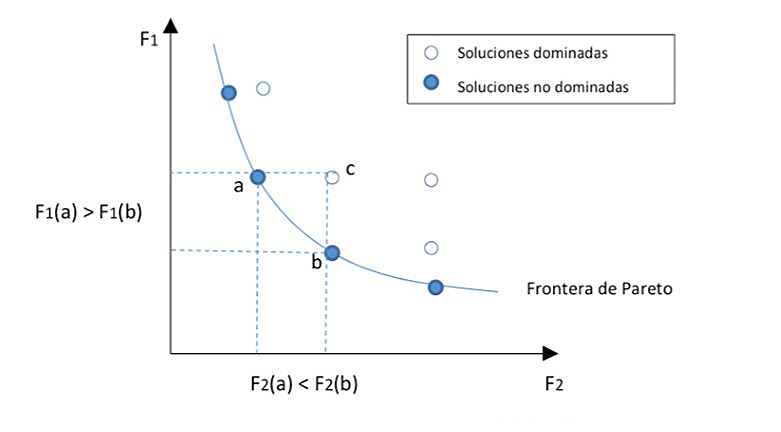
\includegraphics[width=1\textwidth]{/conceptosTeoricos/frentePareto}
	\caption{Frente de pareto en un problema de minimización. Ilustración extraida de~\cite{img:frente_pareto}}
	\label{fig:frentePareto}
\end{figure}